\documentclass[letterpaper, titlepage]{article}
\usepackage[utf8]{inputenc}
\usepackage[spanish, es-tabla]{babel}
\usepackage{graphicx}
\usepackage{amsfonts}
\usepackage{fancyhdr}
\usepackage{mathrsfs}
\usepackage{extarrows}
\usepackage{enumerate}
\usepackage{listings}
\usepackage{anysize, graphicx, color, float, fancyhdr, listings, amsmath, amssymb}
\newcommand{\HRule}{\rule{\linewidth}{0.5mm}}
\newcommand\addtag{\refstepcounter{equation}\tag{\theequation}}

\definecolor{dkgreen}{rgb}{0,0.6,0}
\definecolor{gray}{rgb}{0.5,0.5,0.5}
\definecolor{mauve}{rgb}{0.58,0,0.82}
\definecolor{lgray}{rgb}{0.99,0.97,0.95}
 
\lstset{ %
  language=Matlab,                % the language of the code
  basicstyle=\scriptsize,           % the size of the fonts that are used for the code
  %numbers=left,                   % where to put the line-numbers
  numbers=left,
  numberstyle=\tiny\color{gray},  % the style that is used for the line-numbers
  stepnumber=1,                   % the step between two line-numbers. If it's 1, each line 
                                  % will be numbered
  numbersep=5pt,                  % how far the line-numbers are from the code
  backgroundcolor=\color{lgray},      % choose the background color. You must add \usepackage{color}
  showspaces=false,               % show spaces adding particular underscores
  showstringspaces=false,         % underline spaces within strings
  showtabs=false,                 % show tabs within strings adding particular underscores
  frame=single,                   % adds a frame around the code
  rulecolor=\color{black},        % if not set, the frame-color may be changed on line-breaks within not-black text (e.g. commens (green here))
  tabsize=2,                      % sets default tabsize to 2 spaces
  captionpos=b,                   % sets the caption-position to bottom
  breaklines=true,                % sets automatic line breaking
  breakatwhitespace=false,        % sets if automatic breaks should only happen at whitespace
  %title=\lstname,                   % show the filename of files included with \lstinputlisting;
                                  % also try caption instead of title
  keywordstyle=\color{blue},          % keyword style
  commentstyle=\color{dkgreen},       % comment style
  stringstyle=\color{mauve},         % string literal style
  escapeinside={\%*}{*)},            % if you want to add a comment within your code
  morekeywords={simplify},               % if you want to add more keywords to the set
  inputencoding=utf8,
  extendedchars=true
}
\lstset{literate=
  {á}{{\'a}}1 {é}{{\'e}}1 {í}{{\'i}}1 {ó}{{\'o}}1 {ú}{{\'u}}1
  {Á}{{\'A}}1 {É}{{\'E}}1 {Í}{{\'I}}1 {Ó}{{\'O}}1 {Ú}{{\'U}}1
  {à}{{\`a}}1 {è}{{\`e}}1 {ì}{{\`i}}1 {ò}{{\`o}}1 {ù}{{\`u}}1
  {À}{{\`A}}1 {È}{{\'E}}1 {Ì}{{\`I}}1 {Ò}{{\`O}}1 {Ù}{{\`U}}1
  {ä}{{\"a}}1 {ë}{{\"e}}1 {ï}{{\"i}}1 {ö}{{\"o}}1 {ü}{{\"u}}1
  {Ä}{{\"A}}1 {Ë}{{\"E}}1 {Ï}{{\"I}}1 {Ö}{{\"O}}1 {Ü}{{\"U}}1
  {â}{{\^a}}1 {ê}{{\^e}}1 {î}{{\^i}}1 {ô}{{\^o}}1 {û}{{\^u}}1
  {Â}{{\^A}}1 {Ê}{{\^E}}1 {Î}{{\^I}}1 {Ô}{{\^O}}1 {Û}{{\^U}}1
  {œ}{{\oe}}1 {Œ}{{\OE}}1 {æ}{{\ae}}1 {Æ}{{\AE}}1 {ß}{{\ss}}1
  {ç}{{\c c}}1 {Ç}{{\c C}}1 {ø}{{\o}}1 {å}{{\r a}}1 {Å}{{\r A}}1
  {€}{{\EUR}}1 {£}{{\pounds}}1 {ñ}{{\tilde{n}}}1
}
%\lstset{language=Verilog,caption={Descriptive Caption Text},label=DescriptiveLabel}
%opening

\begin{titlepage}
\title{\begin{minipage}{\textwidth}
\vspace{-9em}
\includegraphics[width=0.2\textwidth]{img/logo_utfsm}
\hfill

\includegraphics[width=0.4\textwidth]{img/logoelo2}
\vspace{1em}
\end{minipage}
%%%%%%%%TÍTULO%%%%%%
\HRule \vspace{1em} \textsc{Laboratorio de Comunicaciones\\ELO-241\\ \Large \vspace{1em} \textbf{Informe Previo 3}\\Modulación Digital de Portadora:\\ASK OOK y BPSK} \HRule \vspace{3em}}
%%%%%%%%NOMBRES%%%%%
\author{\textsl{Andrés Farías Bórquez}\\201121021-2 \and \textsl{Felipe Fernández Pino}\\201121011-5 \and \textsl{Felipe Padilla Oyanader}\\201121037-9}
%%%%%%%%%%%%%%%%%%%%
\date{\vfill \today}
\end{titlepage}
%\tableofcontents
%\listoftables
%\listoffigures

\pagestyle{fancy}
\fancyhead[L]{ELO-241 \begin{minipage}{5em}
\end{minipage}}
\providecommand{\abs}[1]{\lvert#1\rvert}	  

\newcommand{\imagen}[4][0.8]{%[0.8] parámetro por defecto para la escala.
	\begin{figure}[H]\centering
	\includegraphics[width=#1\textwidth]{img/#2}
	\caption{#4}{#3}
	\end{figure}
	}
	%EJEMPLOS
	%"\imagen{007}{\label{fig:007}}{Hola}". Imagen->img/007, con label "fig:007" y descripcion Hola. Escala 0.8.
	%"\imagen[0.5]{007}{fig:007}{Hola}". Mismo anterior, con escala forzada a [0.5] del texto.
	
\newcommand{\bimagen}[6]{%[1] parámetro por defecto para la escala de la minipage.
	\hspace{-0.04\textwidth}
	\begin{minipage}[t]{0.47\textwidth}
	\begin{figure}[H]\centering
	\includegraphics[width=1\textwidth]{img/#1}
	\caption{#3}{#2}
	\end{figure}
	\end{minipage}
	\hfill
	\begin{minipage}[t]{0.47\textwidth}
	\begin{figure}[H]\centering
	\includegraphics[width=1\textwidth]{img/#4}
	\caption{#6}{#5}
	\end{figure}
	\end{minipage}
	\vspace{1em}
}
	
\newcommand{\trimagen}[9]{%[1] parámetro por defecto para la escala de la minipage.
	\hspace{-0.05\textwidth}
	\begin{minipage}[t]{0.3\textwidth}
	\begin{figure}[H]\centering
	\includegraphics[width=1\textwidth]{img/#1}
	\caption{#3}{#2}
	\end{figure}
	\end{minipage}
	\hspace{0.05\textwidth}
	\begin{minipage}[t]{0.3\textwidth}
	\begin{figure}[H]\centering
	\includegraphics[width=1\textwidth]{img/#4}
	\caption{#6}{#5}
	\end{figure}
	\end{minipage}
	\hspace{0.05\textwidth}
	\begin{minipage}[t]{0.3\textwidth}
	\begin{figure}[H]\centering
	\includegraphics[width=1\textwidth]{img/#7}
	\caption{#9}{#8}
	\end{figure}
	\end{minipage}
	\vspace{1em}
}
%EJEMPLO
%\trimagen
%	{imagen1}{\label{fig:1}}
%		{Descripcion1}
%	{imagen2}{\label{fig:2}}
%		{Descripcion2}
%	{imagen3}{\label{fig:3}}
%		{Descripcion3}
\begin{document}
\maketitle
\newpage
\section{Resumen}
	En el desarrollo de este informe previo se describen los métodos de resolución para cada problema, los conceptos teóricos necesarios para comprender cada uno de éstos y se explica el diseño de los módulos de prueba que se pretenden utilizar en esta experiencia.
\section{Objetivos}
	\begin{itemize}
		\item Lograr simular la modulación de señales digitales utilizando transmisión de información en amplitud de portadora (ASK y OOK) y transmisión de información en fase de portadora (BPSK).
		\item Observar los espectros pertenecientes a cada una de estas modulaciones y calcular sus respectivos anchos de banda basándose en tres distintos criterios.
		\item Simular la etapa de demodulación sincrónica para cada una de las señales descritas anteriormente.
		\item Observar y comprender el efecto de introducir un desfase a la señal portadora con la cual se demodula.
		\item Diseñar correctamente un circuito detector de envolvente para frecuencias de portadora dadas.
	\end{itemize}
\newpage

\section{Descripción del Problema}
	En esta sección se procede a identificar cada problema y comprender qué se busca aprender en cada uno.
	\begin{enumerate}
		\item \textbf{Problema 1}
		
			El principal objetivo en este problema es simular correctamente cada una de las modulaciones que se estudian en este experiencia, observando los efectos que producen al modular con señales cuadradas de frecuencia fija y ciclo de trabajo variable o con señales cuadradas pseudoaleatorias (más cercanas a una modulación digital real). Se desea graficar el espectro para cada uno de estos casos identificando diferencias y similitudes.
		\item \textbf{Problema 2}
		
			En este problema se busca determinar el ancho de banda para cada una de las señales moduladas considerando tres distintos criterios:
			\begin{itemize}
				\item Ancho de banda de -3 [dB]
				\item Ancho de banda del primer nulo
				\item Ancho de banda de 98\% de potencia
			\end{itemize}
			
		\item \textbf{Problema 3}
		
			El objetivo de este problema es simular correctamente un demodulador sincrónico junto con un filtro pasa bajos para poder recepcionar los mensajes simulados anteriormente. También se busca determinar el efecto que tiene el demodular con una portadora desfasada desde 0º a 180º.
		\item \textbf{Problema 4}
		
			En este problema busca familiarizarse con el amplificador operacional AD817, entender qué características son las que lo hacen útil para esta experiencia y diseñar las componentes que lo involucran para lograr desfasar la señal portadora.
		\item \textbf{Problema 5}
		
			El objetivo de este problema es lograr diseñar correctamente el circuito detector de envolvente que se emplea para demodular en dos frecuencias de portadora distintas. Se debe especificar qué componentes se utilizan y el rango de voltajes apropiados para el circuito.
	\end{enumerate}
\newpage

\section{Metodología}
	\begin{enumerate}
		\item \textbf{Problema 1}
		
		A traves del uso del software $Matlab$ se procede a simular señales de tipos OOK y BPSK en base a caracteristicas de diseño determinadas observando sus formas de onda y obteniendo el espectro de cada una en base a ciclos de trabajo determinados. Se  analizaran y comentarán cada uno de  los resultados obtenidos.
		\item \textbf{Problema 2}
		
		Se procede a determinar el ancho de banda de las señañes simuladas en el Problema 1 en base a criterios como: Ancho de Banda de Primer Nulo, Ancho de de banda -3dB y ancho de banda en base al 98\% de la Potencia. Se  analizaran y comentarán cada uno de  los resultados obtenidos
		\item \textbf{Problema 3}
		
			Se utiliza el software MATLAB/Simulink para realizar la simulación del circuito demodulador sincrónico.
		\item \textbf{Problema 4}
		
		\item \textbf{Problema 5}
	\end{enumerate}
\newpage
\newpage

\section{Resultados y Contrastaciones}
	\begin{enumerate}
		\item \textbf{Problema 1}
		
		Se procede a elaborar tablas de amplitud de componentes espectrales de señales moduladas digitalemnte mediante OOK y BPSK con los siguientes parámetros:\\
		Para la Señal Portadora:\\
		$Ac=1[V]$\\
		$fc=400[Khz]$\\
		Para la Señal Modulante:\\
		$Am=1[V]$\\
		$fm=5000[Hz]$\\\\
		Para las respectivas simulaciones, se utilizaran los siguientes códigos en $Matlab$:\\
		\subsection{Señal OOK}
		
		\begin{lstlisting}[label=some-code,caption=Codigo Matlab OOK]
		clear all; close all;
		%OOK
		%Caracteristicas: Debe tener un indice de modulacion igual a 1
		Am= 1;
		Ac= 1;
		fm= 5e3; 
		fc= 400e3;
		duty=50;
		syms t;
		%Variables
		wc= 2*pi*fc;
		wm= 2*pi*fm;
		m = (Am/Ac);
		fs= 2*wc;
		%Tiempo
		Tm = (1/fm);
		t = 0:(Tm/1000):1000*Tm;
		%senal Modulante
		E = m.*(square(t.*wm,duty));
		%senal OOK
		f1=(1+E).*cos(t.*wc);
		%Graficos senal OOK
		title('senal OOK')
		subplot(2,1,1);
		A = plot(t,f1);
		grid on;
		set(A,'Color','black','LineWidth',2)
		axis ([0 2*Tm -3.5*m 3.5*m]);
		xlabel('Tiempo[s]')
		ylabel('Voltaje[V]')

		%Grafico senal Modulante
		title('Senal Modulante')
		subplot(2,1,2);
		B = plot(t,E);
		grid on;
		title('Senal Modulante')
		set(B,'Color','red','LineWidth',2)
		set(gca)
		axis ([0 2*Tm -1.5*m 1.5*m]);
		xlabel('Tiempo[s]')
		ylabel('Voltaje[V]')
		\end{lstlisting}
		\newpage
		Se obtienen los siguientes Gráficos:
		
			\trimagen{Senal20_OOK}{\label{fig:sim}}{Señal 20\% ciclo de Trabajo}
			{Senal25_OOK}{\label{fig:sim}}{Señal 25\% ciclo de Trabajo}
			{Senal50_OOK}{\label{fig:sim}}{Señal 50\% ciclo de Trabajo}
			\\
			Cabe destacar la generacion de nulos en la señal dependiendo del ciclo de trabajo de la señal Modulante. La relacion de nulos generados se plantea a traves de :
			\begin{equation}
			T/\tau =n
			\end{equation}
			Donde n es la posicion del Nulo.\\\\
			
		Luego, se implementa el siguiente código para generar los espectros:		
	
	\begin{lstlisting}[label=some-code,caption=Codigo Matlab FFT OOK]
	%%
	%FFT
	close all
	X = fftshift(fft(f1));
	f = fs/2*linspace(-1,1,length(X));
	plot(f,10*log10(abs(X)))
      axis([-5e5 -3e5 0 60])
      [x,y] = ginput(5)
	title('Espectro de senal OOK')
	xlabel('Frecuencia(Hz)')
	ylabel('|Y(f)|')
	\end{lstlisting}
	
	Se obtienen los siguientes espectros:\\
	\trimagen{Esp_OOK_20}{\label{fig:sim}}{Señal 20\% ciclo de Trabajo}
			{Esp_OOK_25}{\label{fig:sim}}{Señal 25\% ciclo de Trabajo}
			{Esp_OOK_50}{\label{fig:sim}}{Señal 50\% ciclo de Trabajo}
	\newpage
				A traves del uso de la funcion $gidinput$ en $Matlab$ se encuentran las respectivas amplitudes y frecuencias fundamentales para cada uno de los espectros. Los valores son:

	\begin{table}[ht]
			\centering
			\begin{tabular}{c c c c c}
				Nº armónica & Frecuencia $\cdot$ 1.0e+05 [Hz] & Potencia [dB]\\
				\hline
				1 & -4.0207 & 57.6316  \\
				2 & -4.0714 & 49.7368   \\
				3 & -3.9700 & 49.5614   \\
				4 & -4.1221 & 48.8596   \\
				5 & -3.9194 & 48.6842  
			\end{tabular}
			\caption{Valores frecuencias fundamentales OOK}
			\label{tab:tabla1}
		\end{table}

	\newpage	
	\subsection{Señal BPSK}
	\begin{lstlisting}[label=some-code,caption=Codigo Matlab BPSK]
	%Experiencia 3
		clear all; close all;
		%BPSK
		%Caracteristicas: Debe tener un indice de modulacion igual a 1
		Am= 1;
		Ac= 1;
		fm= 5e3; 
		fc= 400e3;
		duty=50;
		syms t;
		%Variables
		wc= 2*pi*fc;
		wm= 2*pi*fm;
		m = (Am/Ac);
		fs= 2*wc;
		%Tiempo
		Tm = (1/fm);
		t = [0:(Tm/1000):1000*Tm];
		%senal Modulante
		E = (0.5+0.5.*square(t.*wm,duty));
		%senal ASK
		f1=cos(t.*wc + 180.*E);
		%Graficos senal BSK
		title('senal BPSK')
		subplot(2,1,1);
		A = plot(t,f1);
		grid on;
		set(A,'Color','black','LineWidth',2)
		axis ([0 2*Tm -3.5*m 3.5*m]);
		xlabel('Tiempo[s]')
		ylabel('Voltaje[V]')

		%Grafico senal Modulante
		title('Senal Modulante')
		subplot(2,1,2);
		B = plot(t,E);
		grid on;
		title('Senal Modulante')
		set(B,'Color','red','LineWidth',2)
		set(gca)
		axis ([0 2*Tm -0.5*m 1.5*m]);
		xlabel('Tiempo[s]')
		ylabel('Voltaje[V]')
		\end{lstlisting}
	
	Se obtienen los siguientes gráficos:\\
	\trimagen{Senal20_BPSK}{\label{fig:sim}}{Señal 20\% ciclo de Trabajo}
			{Senal25_BPSK}{\label{fig:sim}}{Señal 25\% ciclo de Trabajo}
			{Senal50_BPSK}{\label{fig:sim}}{Señal 50\% ciclo de Trabajo}\\
			Es notorio en cada grafico la relacion de cambio de fase cada vez que la señal modulante cambia entre valores discretos, lo cual corresponde a una definicion directa de señales tipo BPSK.
	\newpage
	Luego se implementa el siguiente codigo $Matlab$ para generar los espectros:
	
	\begin{lstlisting}[label=some-code,caption=Codigo Matlab FFT BPSK]
	%%
	%FFT
	close all
	X = fftshift(fft(f1));
	f = fs/2*linspace(-1,1,length(X));
	plot(f,10*log10(abs(X)))
      axis([-5e5 -3e5 0 60])
      [x,y] = ginput(5)
	title('Espectro de senal BPSK')
	xlabel('Frecuencia(Hz)')
	ylabel('|Y(f)|')
	\end{lstlisting}
	
	Se obtienen los siguientes Espectros:\\
	\trimagen{Esp1_BPSK_20}{\label{fig:sim}}{Señal 20\% ciclo de Trabajo}
			 {Esp1_BPSK_25}{\label{fig:sim}}{Señal 25\% ciclo de Trabajo}
			 {Esp1_BPSK_50}{\label{fig:sim}}{Señal 50\% ciclo de Trabajo}\\
			 Las principales diferencias encontradas
			 
			 Luego, se obtienen las siguientes tablas de datos:
			 
			\begin{table}[ht]
			\centering
			\begin{tabular}{c c c c c}
				Nº armónica & Frecuencia $\cdot$ 1.0e+05 [Hz] & Potencia [dB]\\
				\hline
				1 & -4.0219 & 45.0000  \\
				2 & -4.0726 & 41.8421   \\
				3 & -3.9712 & 42.0175   \\
				4 & -4.1210 & 41.1404   \\
				5 & -3.9205 & 40.6140  
			\end{tabular}
			\caption{Valores frecuencias fundamentales BPSK}
			\label{tab:tabla1}
		\end{table}
		
	\newpage
		\item \textbf{Problema 2}
		
		Se procede a calcular analiticamente los anchos de banda para cada uno de los casos anteriores. Para ello se utilizarán graficas espectrales mediante matlab dependiendo del criterio de determinacion de Bandwith pedido.
		\subsection{Ancho de Banda -3dB}
			\subsubsection{Señal OOK}
		Se obtienen los siguientes espectros en base a una caida de -3dB:\\
	\trimagen{BW_3db_OOK_20}{\label{fig:sim}}{Señal 20\% ciclo de Trabajo}
			 {BW_3db_OOK_25}{\label{fig:sim}}{Señal 25\% ciclo de Trabajo}
			 {BW_3db_OOK_50}{\label{fig:sim}}{Señal 50\% ciclo de Trabajo}\\
			\begin{table}[ht]
			\centering
			\begin{tabular}{c c c c c}
				Armonica & Ciclo de Trabajo & Frecuencia Armónica $\cdot$ 1.0e+05[Hz] & Potencia [dB]\\
				\hline
				1 & 20 & -4.0207 & 56.7544  \\
				3 & 20 & -4.1728 & 50.2632	\\
				1 & 25 & -4.0207 & 53.9474   \\
				3 & 25 & -4.1728 & 48.5088   \\
				1 & 50 & -4.0207 & 52.8947  \\
				3 & 50 & -4.1728 & 49.9123   \\
			\end{tabular}
			\caption{Caida de -3dB}
			\label{tab:tabla1}
		\end{table}	
		
		\begin{table}[ht]
			\centering
			\begin{tabular}{c c c c c}
				Ciclo de Trabajo & Ancho de banda$\cdot$ 1.0e+05[Hz] \\
				\hline
				20 & 0.1521   \\
				25 & 0.1521  \\
				50 & 0.1521   \\
			\end{tabular}
			\caption{Anchos de Banda de Señales para Diversos ciclos de Trabajo}
			\label{tab:tabla1}
		\end{table}
				
			\subsubsection{Señal BPSK}
		Se obtienen los siguientes espectros en base a una caida de -3dB:\\
	\trimagen{BW_3db_BPSK_20}{\label{fig:sim}}{Señal 20\% ciclo de Trabajo}
			 {BW_3db_BPSK_25}{\label{fig:sim}}{Señal 25\% ciclo de Trabajo}
			 {BW_3db_BPSK_50}{\label{fig:sim}}{Señal 50\% ciclo de Trabajo}\\	
			 		
			\begin{table}[ht]
			\centering
			\begin{tabular}{c c c c c}
				Armonica & Ciclo de Trabajo & Frecuencia Armónica $\cdot$ 1.0e+05[Hz] & Potencia [dB]\\
				\hline
				1 & 20 & -4.0242 & 55.7018  \\
				2 & 20 & -4.0726 & 51.4912	\\
				1 & 25 & -4.0242 & 55.3509   \\
				2 & 25 & -4.0726 & 52.1930   \\
				1 & 50 & -4.0242 & 54.4737  \\
				3 & 50 & -4.1694 & 49.0351   \\
			\end{tabular}
			\caption{Caida de -3dB}
			\label{tab:tabla1}
		\end{table}				

		\begin{table}[ht]
			\centering
			\begin{tabular}{c c c c c}
				Ciclo de Trabajo & Ancho de banda$\cdot$ 1.0e+05[Hz] \\
				\hline
				20 & 0.0519  \\
				25 & 0.0484	  \\
				50 & 0.1452   \\
			\end{tabular}
			\caption{Anchos de Banda de Señales para Diversos ciclos de Trabajo}
			\label{tab:tabla1}
		\end{table}			
			
			
		\subsection{Ancho de Banda Primer Nulo}
			\subsubsection{Señal OOK}
			Se obtienen los siguientes Espectros en base al primer nulo:\\
	\trimagen{BW_null_OOK_20}{\label{fig:sim}}{Señal 20\% ciclo de Trabajo}
			 {BW_null_OOK_25}{\label{fig:sim}}{Señal 25\% ciclo de Trabajo}
			 {BW_null_OOK_50}{\label{fig:sim}}{Señal 50\% ciclo de Trabajo}\\
			 
		
		\begin{table}[ht]
			\centering
			\begin{tabular}{c c c c c}
				$Numero$ Nulo & Ciclo de Trabajo & Frecuencia Nulos $\cdot$ 1.0e+05[Hz] & Potencia [dB]\\
				\hline
				1 & 20 & -4.2742 & 19.7368  \\
				2 & 20 & -3.7719 & 20.4386	\\
				1 & 25 & -3.8180 & 20.9649   \\
				2 & 25 & -4.2235 & 19.7368   \\
				1 & 50 & -4.1221 & 18.8596  \\
				2 & 50 & -3.9194 & 21.3158   \\
				
			\end{tabular}
			\caption{Nulos señales OOK a diversos ciclos de trabajo}
			\label{tab:tabla1}
			
		\end{table}
		\begin{center}
		Finalmente los anchos de banda respectivos para cada señal quedan denotados por:
		\end{center}

		\begin{table}[ht]
			\centering
			\begin{tabular}{c c c c c}
				Ciclo de Trabajo & Ancho de banda$\cdot$ 1.0e+05[Hz] \\
				\hline
				20 & 0.5023   \\
				25 & 0.4055	  \\
				50 & 0.2027   \\
			\end{tabular}
			\caption{Anchos de Banda de Señales para Diversos ciclos de Trabajo}
			\label{tab:tabla1}
		\end{table}
		
		\subsubsection{Señal BPSK}
			Se obtienen los siguientes Espectros en base al primer nulo:\\
	\trimagen{BW_null_BPSK_20}{\label{fig:sim}}{Señal 20\% ciclo de Trabajo}
			 {BW_null_BPSK_25}{\label{fig:sim}}{Señal 25\% ciclo de Trabajo}
			 {BW_null_BPSK_50}{\label{fig:sim}}{Señal 50\% ciclo de Trabajo}\\
			 
			 \begin{table}[ht]
			\centering
			\begin{tabular}{c c c c c}
				$Numero$ Nulo & Ciclo de Trabajo & Frecuencia Nulos $\cdot$ 1.0e+05[Hz] & Potencia [dB]\\
				\hline
				1 & 20 & -4.2592 & 7.4561  \\
				2 & 20 & -3.7546 & 6.7544	\\
				1 & 25 & -4.2108 & 7.8070  \\
				2 & 25 & -3.8030 & 7.1053   \\
				1 & 50 & -4.1071 & 6.9298   \\
				2 & 50 & -3.9067 & 7.4561   \\
				
			\end{tabular}
			\caption{Nulos señales BPSK a diversos ciclos de trabajo}
			\label{tab:tabla1}
		\end{table}
		
		\begin{center}
		Finalmente los anchos de banda respectivos para cada señal quedan denotados por:
		\end{center}

		\begin{table}[ht]
			\centering
			\begin{tabular}{c c c c c}
				Ciclo de Trabajo & Ancho de banda$\cdot$ 1.0e+05[Hz] \\
				\hline
				20 & 0.5046   \\
				25 & 0.4078	  \\
				50 & 0.2004   \\
			\end{tabular}
			\caption{Anchos de Banda de Señales para Diversos ciclos de Trabajo}
			\label{tab:tabla1}
		\end{table}	

		\subsubsection{Determinacion Ancho de Banda 98\% Potencia}
			Para determinar analiticamente el 98\% de potencia de una señal se utilizará calculo de 			coeficientes de la Serie de Fourie. Sea una resistencia de $50[\Omega]$, la potencia total disipada en ella tiene un valor de:
			
		\begin{equation}	
	P_{av}={1 \over 2 \cdot 50}(A^{2}+B^{2})[W]
		\end{equation}
		
		
	Con A= Amplitud Señal Modulante y B= Amplitud Señal Portadora	
		
		\item \textbf{Problema 3}
		
		\item \textbf{Problema 4}
		
		Se tiene el siguiente circuito desfasador mostrado a continuación:
		
\begin{figure}[H]
  \centering
    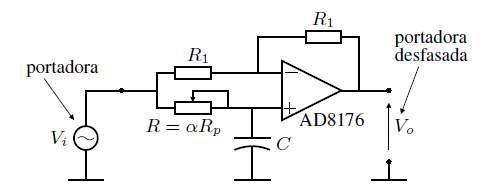
\includegraphics[width=0.6\textwidth]{circuitdesf}
  \caption{Circuito Desfasador.}
  \label{fig:ejemplo}
\end{figure}

		
Para comenzar entenderemos cuales son las caracteristicas que hacen del amplificador operacional AD817 util en esta experiencia,siendo una de estas su ancho de banda unitaria el cual es de 50[Mhz] lo que quiere decir que dentro de este rango de frecuencias no se presentaran atenuaciones en la señal de salida, como en este caso se utilizara una frecuencia de portadora de $f_{c} = 400[kHz]$ el amplificador operacional no causara problema a la señal de salida.

Otra característica importante es el slew rate el cual en el AD817 es de $350[\frac{V}{\mu s}]$ , el slew rate es la máxima velocidad de cambio que puede tener la señal de salida, es decir la capacidad del A.O para seguir los cambios de una señal de alta frecuencia de entrada y que la señal de salida no presente problemas.

En conclusión estas caracteristicas del AD817 hace posible el procesamiento de señales de entrada de alta velocidad siendo algunos ejemplos las señales de imágenes y videos, y en este caso la modulación de alta frecuencia.

Ahora para diseñar los valores de $ R_{p} $ y $C$ se tiene que la función de transferencia  del circuito desfasador es la siguiente:

\begin{equation}
V_{o} = V_{i} \frac{1- j \omega R C}{1 + j \omega R C}
\end{equation}
		
En donde expresando el fasor en modulo y ángulo se tiene:

\begin{equation*}
\abs{V_{o}}  = \abs{V_{i}} \sqrt{\frac{1 +( \omega R C)^2}{1 +( \omega R C)^2}} \frac{\angle \arctan(- \omega R C ) }{\angle \arctan(\omega R C )}
\end{equation*}

\newpage

Dado que la arcotangente es una función impar finalmente se obtiene:

\begin{equation}
\abs{V_{o}}  = \abs{V_{i}} \angle -2 \arctan (\omega R C)
\end{equation}
		
Se observa que no importa la frecuencia o valores de R y C la amplitud de la señal salida es igual al de la entrada, ahora tomando el ángulo se tiene:	

\begin{align*}
\theta & = -2 \arctan (\omega R C) \\
R & = \frac{\tan( -\theta/2)}{ \omega C }\\
\end{align*}

Dado que $- \frac{\pi}{2}< \theta < 0$ 	buscamos el desfase para $\theta =- \frac{\pi}{2}$ Remplazando este valor en la ecuación se obtiene:

\begin{equation}
R = \alpha R_{p} = \frac{1}{\omega C}
\end{equation}

Escogiendo para este valor de desfase,el valor máximo del potenciometro y con $f_{c}= 400[kHz]$ se tiene

\begin{align*}
\alpha & = 1 \\
\omega & = 2 \pi f_{c} = 2.513.274 [\frac{rad}{s}] \\
\end{align*}

Fijando el potenciometro de $ R=2[k \Omega ] $ se tendra un valor de $ C = 0.198[nF] $.

Finalemte con respecto a $ R_{1} $ se escoge un valor de unos pocos $ k \Omega $ con el fin de reducir el efecto ocasionado por las capacitancias parasitas, las cuales provocan oscilaciones de alta frecuencia en el lazo cerrado. 

Luego los valores diseñados son:

\begin{align*}
R & = 2[k \Omega] \\
R_{1} & = 10[k \Omega] \\
C & = 0.198[nF] \\
\end{align*}

\newpage

\item \textbf{Problema 5}

Para diseñar el circuito detector de envolvente se basa en el siguiente criterio de diseño:

\begin{equation}
 \frac{1}{f_{p}} \ll \tau \ll \frac{1}{f_{m}}
\end{equation}

En donde la constante de tiempo es $\tau = RC$

Este criterio se dene a que eligiendo un valor muy pequeño de $\tau$ cercano a $1/fp$ existirá un ripple muy pronunciado debido a la rapidez que tendrá el comportamiento dinámico del circuito impediendo la deteccion correcta de la envolvente, por otro lado el valor pequeño de $tau$ producira que el efecto llamado negative peak cliping el cual consiste en que la señal demodulada tiende a redondear y no seguir correctamente a la señal AM será menos significativa.

En la siguiente figura se ilustran estos efectos.	
		
\begin{figure}[H]
  \centering
    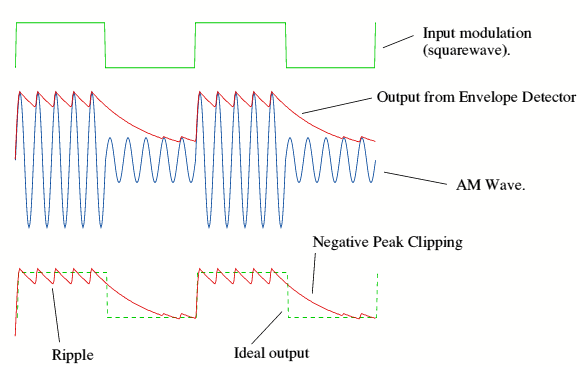
\includegraphics[width=0.7\textwidth]{demodulacion1}
  \caption{Efectos Ripple y Negative peak clipping.}
  \label{fig:ejemplo}
\end{figure}


Por otro lado si escogemos un valor de $tau$ más grande el efecto ripple será menos notorio, pero por otro lado el efecto del negative peak clipping se verá incrementado por lo cual usando las inecuaciones (4) consideraremos componentes con valores tales que la constante de tiempo se encuentre en un equilibrio 
para que no exista ni un efecto Ripple pronunciado ni un negative peak clipping pronunciado y obtener una demodulacion bastante correcta de la señal AM.
\newpage
Considerando $ f_{m} = 10[kHz] $ y $ f_{c} = 400[kHz] $ resolviendo se tiene:

\begin{align*}
\frac{1}{f_{p}}& \ll \tau \ll  \frac{1}{f_{m}} \\
2,5\cdot10^{-6} [s] &  \ll RC \ll  1\cdot10^{-4} [s] \\
\end{align*}

Considerando $ R = 10[k \Omega] $:

\begin{equation}
0.25[nF]   \ll C \ll  10[nF]
\end{equation}

Escogiendo $ C = 5.6[nF] $ y simulando:

\begin{figure}[H]
  \centering
    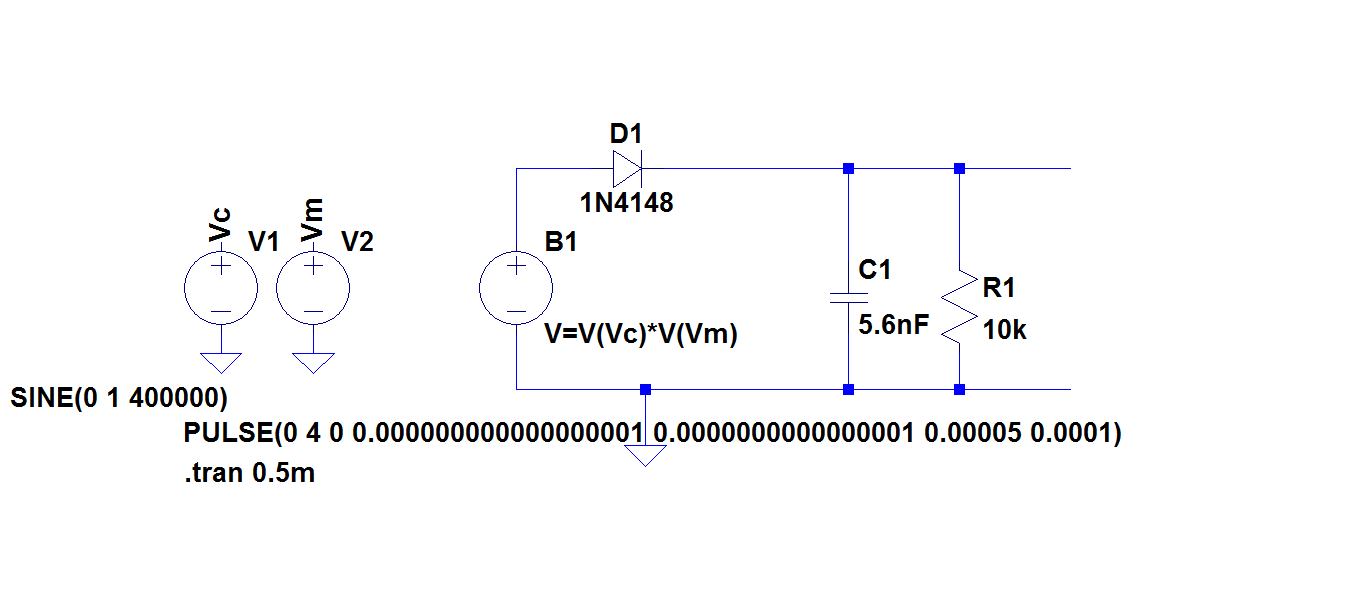
\includegraphics[width=0.8\textwidth]{circuitosim}
  \caption{Circuito simulado mediante LTspice.}
  \label{fig:ejemplo}
\end{figure}

\begin{figure}[H]
  \centering
    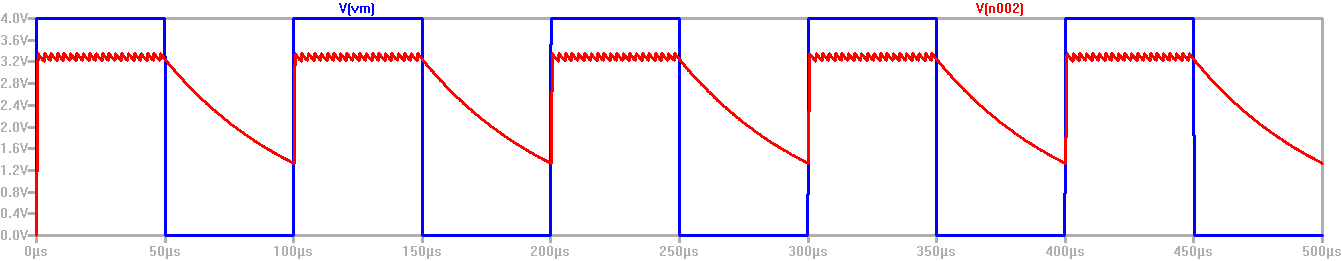
\includegraphics[width=0.8\textwidth]{graficodemod}
  \caption{Señal moduladora cuadrada y señal demodulada.}
  \label{fig:ejemplo}
\end{figure}

En la figura se observa  que la señal demodulada  se observa cómo se encuentran presentes ambos efectos explicados anteriormente pero ni uno de los es tan imponente como para afectar la finalidad del circuito que es la detección de envolvente. Además se observa menos voltaje en la señal de salida esto se debe a la caída de tensión que existe en el diodo.
\newpage
El diodo que se utilizara es el 1N4148 el cual es un con alta velocidad de switching de frecuencia máxima de 250[MHz], por lo cual para nuestra señal AM de 400[kHz] es más que suficiente , NO SEGURO EN ALGUNOS LADOS SALE 100 MEGAS   
\end{enumerate}
\newpage



\section{Conclusiones}
	\begin{itemize}
		\item Conclusión
		\item Conclusión
	\end{itemize}
\end{document}